% 原文 pp.73–79（印刷 pp.1191–1197）

% ===== 原文 p.73 =====
\subsection{纯规范理论}
% 原文 §5.5：Pure gauge theory

我们还需要确定有效作用量为（5.20）的那个理论的量子行为。为此，我们先通过分析二维的纯规范理论（pure gauge theory）来作练习，它的作用量是（5.20）前两项之和。这是一个我们以后会从许多不同角度重新回到的问题，例如在第 11 讲中。

我们不妨考虑任一连通紧 Lie 群 $G$。（5.20）第一项中的范数由一个 $G$ 上的双不变度量（bi-invariant metric）定义。我们在周长为 $V$（=体积）的圆 $S^1_V$ 上量子化这个理论。一般地，要在 $n$ 维流形 $Y$ 上量子化一个 $n$ 维规范理论，我们考虑 $\mathbb{R}\times Y$ 上处于时间规范（temporal gauge）的联络，并取运动方程的解模去与时间无关的规范变换。对于不含 $\theta$ 项的纯规范理论，所得的空间是 $Y$ 上联络空间模规范变换之后的（余）切丛（(co)tangent bundle）。对于 $Y=S^1_V$，我们先固定一个基点；于是模规范等价的联络由和乐（holonomy）——即 $G$ 的一个元素——所指定。改变基点会把和乐共轭，因此量子 Hilbert 空间是
\[
  \mathcal{H}_{\mathrm{gauge}}(\theta=0)=L^2(G)^G,
\]
也就是 $G$ 上共轭不变函数构成的空间。这个空间的一组基是不可约表示的特征标（character）的集合。

接下来我们计算 Hamilton 量。设 $A_t=A_t(x)dx$ 是 $\mathbb{R}\times S^1_V$ 上的一个联络（坐标为 $t,x$），处于时间规范，相对于某个平凡化；又设 $g_t\in G$ 为相应的和乐路径。在 $A_t$ 为常数的规范中，我们有 $g_t=e^{VA_t}$。于是作用量（5.20）中的第一项是
\begin{equation}
  \tag{5.23}
  \label{eq:5-23}
  \frac{N}{2e^2}\iint\left|\frac{dA}{dt}\right|^2 dtdx=\frac{N}{2e^2V}\int|\dot g|^2dt.
\end{equation}

% [Tutor Note: 由 (5.23) 左边到右边用了两件事，值得逐步核对：其一，$A_t$ 与 $x$ 无关，故 $\int_{S^1_V}dx\,|\dot A|^2=V|\dot A|^2$；其二，$g_t=e^{VA_t}$ 给出 Lie 代数元 $\dot g\,g^{-1}=V\dot A$，这里 $|\dot g|^2$ 指的是双不变度量作用在右不变速度 $\dot g g^{-1}\in\mathfrak{g}$ 上的模方，而不是把 $g$ 当作矩阵后逐元求导的 $\operatorname{tr}(\dot g^2)$。由此 $|\dot g|^2=V^2|\dot A|^2$，两边恰好相等。$1/V$ 因子正是「质量 $\propto V$」的来源，若把 $|\dot g|^2$ 误解为 $\operatorname{tr}\dot g^2$，就会丢掉整个 $V$ 依赖，进而把 (5.24) 的谱算错。]

这正是一个质量为 $N/e^2V$ 的经典粒子在 Riemann 流形 $G$ 上运动时的 Lagrange 量；相应的量子 Hamilton 量为
\begin{equation}
  \tag{5.24}
  \label{eq:5-24}
  H_{\mathrm{gauge}}=\frac{e^2V}{2N}\Delta_G,
\end{equation}
其中 $\Delta_G$ 是 $G$ 上的 Laplace 算子。其本征函数是不可约表示的特征标，本征值与 Casimir 成正比。

% [Tutor Note: (5.24) 中 $\Delta_G$ 的符号约定必须与「本征值正比于 Casimir」相容。几何学家惯用的 Laplace–Beltrami 算子 $\Delta=-\operatorname{div}\nabla$ 是正算子，其本征值即 Casimir（对 $SU(2)$ 的 spin-$j$ 表示为 $j(j+1)$）；而分析学家常写的 $\Delta=\operatorname{div}\nabla$ 是负算子。若误取后者，(5.24) 便给出负定的 Hamilton 量，真空不稳。此处 $H_{\rm gauge}$ 无负号，等价于声明 $\Delta_G\ge0$。同一约定下，$G$ 上的自由粒子能量按 $e^2V/2N$ 整体标度——这正是大 $V$ 时能级间距变稀的原因。]

现在考虑（5.20）中的 $\theta$ 项。对于 $G=U(k)$，我们有一个自然的闭虚 1-形式 $\alpha\in i\Omega^1_G$，它就是 Maurer–Cartan 形式的迹。于是用和乐路径 $g_t$ 来表达，作用量中的 $\theta$ 项为
\begin{equation}
  \tag{5.25}
  \label{eq:5-25}
  \frac{\theta}{2\pi}\int g^{*}\alpha.
\end{equation}
这是一个拓扑项（topological term）——它在路径 $g_t$ 的重参数化下不变。更几何地说，$\theta\alpha$ 是 $G$ 上一个拓扑平凡的厄米线丛（Hermitian line bundle）$L_\theta$ 上的平坦联络（flat connection），并且模等价地由 $H^1(G;\mathbb{T})$ 中的一个元素给出。于是（5.25）就是这个平坦丛中的平行移动。\footnote{一般地，当流形带边界时——此处是区间——经典场论的作用量不是一个数，但我们在这里不强调这一点。}更一般地，我们可以用任意一个带联络的厄米线丛 $L$ 来「扭化」（twist）我们的力学系统。

% ===== 原文 p.74 =====
量子 Hilbert 空间是 $L$ 的截面构成的空间，而 Hamilton 量取为作用在这些截面上的 Laplace 算子。在我们的情形中得到空间
\[
  \mathcal{H}_{\mathrm{gauge}}(\theta)=L^2(G,L_\theta)^G,
\]
即不变截面构成的空间，其 Hamilton 量为（5.24）。对任意的 $G$，元素 $e^{i\theta}\in H^1(G;\mathbb{T})$ 对应于一个同态 $e^{i\theta}:\pi_1G\to\mathbb{T}$。回想 $\pi_1G$ 是 $G$ 的中心的子群。于是，作用在 $\mathcal{H}_{\mathrm{gauge}}(\theta)$ 上的 Laplace 算子的本征函数，是 $G$ 的单连通覆盖群（covering group）的这样一些表示的特征标：它们限制到 $\pi_1G$ 上等于 $e^{i\theta}$；本征值仍与 Casimir 成正比。

对于酉群 $G=U(k)$，我们像以前一样把 $\theta$ 等同于 $\mathbb{R}/2\pi\mathbb{Z}$ 中的元素。最小的 Casimir 出现在表示 $\det^{\tilde\theta/2\pi}$ 上，其中 $\tilde\theta\in\mathbb{R}$ 是 $\theta$ 的绝对值最小的代表元。若 $\theta\neq\pi$，这样的 $\tilde\theta$ 是唯一的；但 $\theta=\pi$ 时有两种可能：$\tilde\theta=\pi$ 与 $\tilde\theta=-\pi$。对于 $G=SO(k)$，其单连通覆盖是 $\tilde G=\mathrm{Spin}(k)$。$\theta=0$ 时有唯一的最低表示，即 $SO(k)$ 的平凡表示。$\theta=\pi$ 时，最低表示在 $k$ 为奇数时是旋量表示，在 $k$ 为偶数时是两个半旋量表示。在大体积极限下只有最低本征值存活下来，于是当 $\theta=\pi$ 时，在复的情形（$U(k)$）下我们有两个真空，而在实的情形（$SO(k)$）下当 $k$ 为偶数时有两个真空。注意在这些情形下，两个真空在对合 $g\mapsto-1\cdot g$ 下相互对应。（还请注意，$L_{\theta=0}$ 这个丛是实的。）我们将看到，当我们加入物质之后，这一真空结构依然保持。因此，对 $G=U(k)$ 与 $G=SO(2\ell)$，宇称对称性（parity symmetry，见（5.4））在 $\theta=\pi$ 处自发破缺。这回答了我们第三个问题。

% [Tutor Note: 说「最小的 Casimir 出现在 $\det^{\tilde\theta/2\pi}$ 上」时，作者的隐含前提是：$\pi_1(U(k))=\mathbb{Z}$ 而 $H^1(G;\mathbb T)$ 的分类要求该表示的权（此处即行列式的幂次）必须恰为 $\tilde\theta/2\pi$，才能把扭化丛 $L_\theta$ 的作用吸收掉。$U(k)$ 的不可约表示由最高权标号，其 Casimir 随标号二次增长，故 $|m|$ 最小的那个（$m=\tilde\theta/2\pi$，即行列式的幂）Casimir 最小；$\theta=\pi$ 时 $\tilde\theta=\pm\pi$ 给出 $m=\pm1/2$ 两个同等最低的表示，这正是「两个真空」的代数来源。若误以为可以对任 $m$ 取最低，就会漏掉 $\theta$ 的 $2\pi$ 周期性。]

当体积 $V\to\infty$ 时，（5.24）的本征值变得彼此分得很开。特别地，在无穷体积极限下，真空之上不存在有限能量的态（或者在少数我们会遇到两个简并真空的特殊情形下，那些真空之上也不存在）。所以无穷体积下的物理 Hilbert 空间只包含真空（或诸真空）——$\mathbb{R}^2$ 上的纯规范理论是平凡的。

现在取 $G=U(1)$。于是真空能量密度（vacuum energy density），即 Hamilton 量（5.24）的最小本征值除以体积 $V$，为
\begin{equation}
  \tag{5.26}
  \label{eq:5-26}
  E_{\mathrm{vac}}(\theta)=\frac{e^2}{2N}\min_{n\in\mathbb{Z}}\left(n-\frac{\theta}{2\pi}\right)^2.
\end{equation}
请注意，$E_{\mathrm{vac}}$ 除 $\theta=\pi$ 之外处处光滑；在 $\theta=\pi$ 处它的导数有间断。

% [Tutor Note: (5.26) 中 $\min_n$ 的取到者随 $\theta$ 变化，这就是「$E_{\rm vac}$ 只在 $\theta=\pi$ 处不光滑」的全部内容：对 $|\theta|<\pi$ 极小由 $n=0$ 给出，$E_{\rm vac}=e^2\theta^2/8\pi^2N$；越过 $\theta=\pi$ 后极小改由 $n=1$（或 $-1$）给出，两条抛物线在 $\theta=\pi$ 处相交成尖点，左右导数分别为 $\pm e^2/4\pi N$，并不相等。$\theta=\pi$ 时 $n=0$ 与 $n=1$ 两个极小简并，正是正文所说「两个真空」以及宇称自发破缺的根源；这也解释了为何下面的 (5.27) 在 $\theta=\pi$ 处给出双倍的配分函数。]

对于 $G=U(k)$，公式（5.26）只需乘以 $k$。

对于 $\Sigma=[0,T]\times S^1_V$，纯规范理论的配分函数 $Z_\Sigma(\theta)$ 有如下 Hilbert 空间解释
\[
  Z_\Sigma(\theta)\sim\langle\Omega|e^{-TH(\theta)}|\Omega\rangle\qquad\text{当 }T\to\infty,
\]
其中 $H(\theta)$ 是 Hamilton 量，$\Omega$ 是真空。对纯规范理论，由（5.26）对 $G=U(1)$ 得到
\begin{equation}
  \tag{5.27}
  \label{eq:5-27}
  Z_\Sigma(\theta)\sim\exp\left(cTV-\frac{e^2TV}{2N}\min_{n\in\mathbb{Z}}\left(n-\frac{\theta}{2\pi}\right)^2\right)\qquad\text{当 }T\to\infty.
\end{equation}
这里 $c$ 是一个常数，它代表着路径积分的不确定性，等价地说，代表着我们可以自由地在 Hamilton 量上加上一个常数（与 $\theta$ 无关），从而改变 Hamilton 量。

% ===== 原文 p.75 =====
这与来自瞬子（instanton）求和的预言（5.3）相当不同。注意，由于 $\sigma$ 模型的经典共形不变性，推导（5.3）时所用的那些瞬子并没有确定的尺度；它们可以被重新标度。正因如此，瞬子求和在长距离上并不可靠。无论如何，（5.27）回答了纯规范理论的问题 2。它同时也给出了到 Grassmann 流形的 $\sigma$ 模型的答案，因为这个模型在长距离上与纯规范理论非常相似。

\subsection{二维经典电磁学}
% 原文 §5.6：Classical electromagnetism in two dimensions

在分析带玻色物质的量子规范理论——即作用量（5.20）中的 $\phi$ 场——之前，我们先讨论经典物理。作为经典分析，我们在 $G=U(1)$ 理论中工作。纯规范理论的经典方程——Maxwell 方程——是
\begin{equation}
  \tag{5.28}
  \label{eq:5-28}
  \frac{N}{e^2}d^{*}_{A}F_{A}=0.
\end{equation}
由于我们处在两个时空维中，这意味着电场 $f=f_A={*}F_A$ 是一个常数。以「$x$」记空间坐标，它不过是 $\mathbb{R}$ 的一个拷贝。在 $x=x_0$ 处放置一个电荷为 1 的点电荷。于是作为 $x$ 的函数的电场 $f$ 满足带有一个由电荷给出的右端的（5.28）：
\[
  \frac{N}{e^2}\frac{df}{dx}=-\delta(x-x_0).
\]
因此，电场的值在穿过一个电荷时跳跃 $-e^2/N$。（见 Figure 5.4。）考虑到许多电荷，并假定它们都是基本电荷的整数倍（这是量子理论的一个结论），我们看到
\begin{equation}
  \tag{5.29}
  \label{eq:5-29}
  \theta=\frac{2\pi Nf}{e^2}\in\mathbb{R}/2\pi\mathbb{Z}
\end{equation}
是一个常数。所以在经典理论中（在假定电荷量子化的前提下）存在一个角（angle，此处即后文所称的 $\theta$ 角）。

\begin{figure}[htbp]
  \centering
  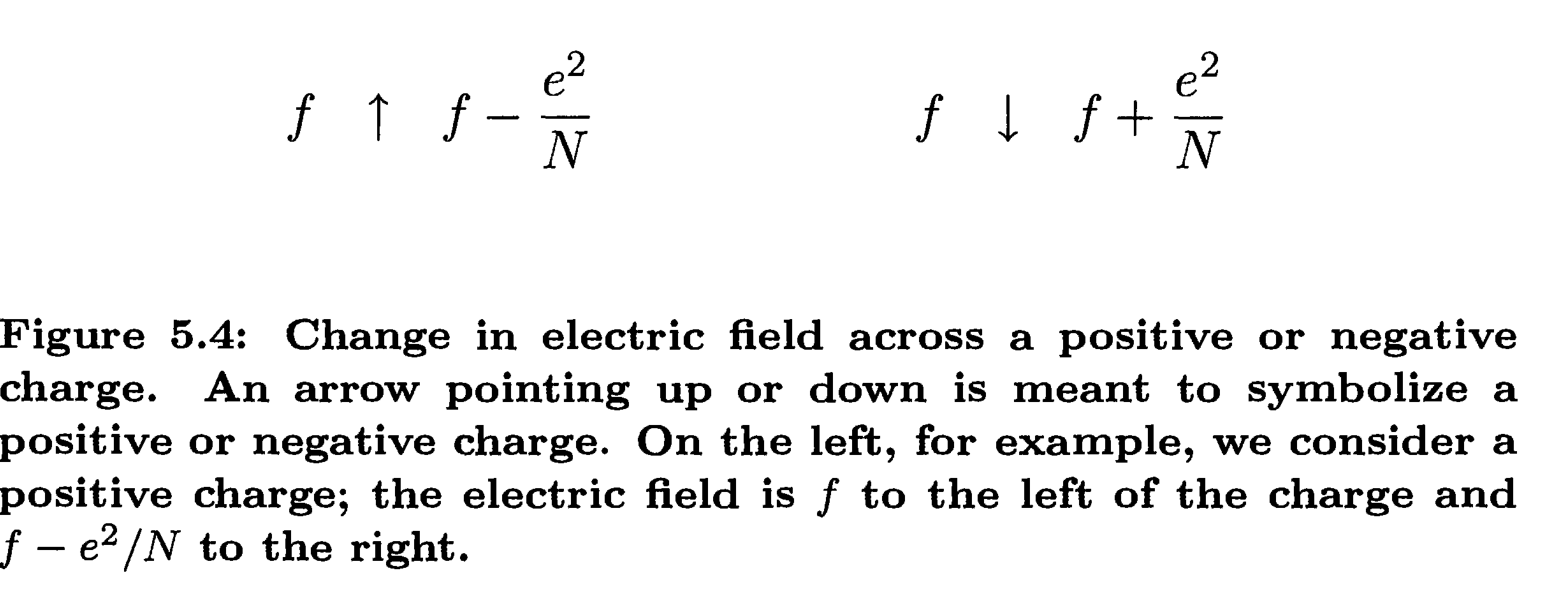
\includegraphics[width=0.76\textwidth]{figs/fig_p075_1.png}
  \caption{电场穿过一个正电荷或负电荷时的改变。向上或向下的箭头用以象征正电荷或负电荷。例如左图考虑的是正电荷：电场在电荷左侧为 $f$，在右侧为 $f-e^2/N$。（原文 Figure 5.4，p.75）}
  \label{fig:p075-1}
\end{figure}

% [Tutor Note: (5.29) 把 $\theta$ 定义为 $2\pi Nf/e^2$，其中 $f=*F_A$ 的符号依赖于二维时空的定向。用「正电荷使 $f$ 向右跳跃 $-e^2/N$」这一条（即 Gauss 定律 $\frac{N}{e^2}\partial_x f=-\rho$）可以核对系数：设 $f(-\infty)=f_0$ 而总电荷为 $Q=\int\rho\,dx$，则 $f(+\infty)=f_0-e^2Q/N$，于是 $\theta(+\infty)-\theta(-\infty)=-2\pi Q$。这既说明 $\theta$ 只有在电荷量子化（$Q\in\mathbb{Z}$）时才良定义于 $\mathbb{R}/2\pi\mathbb{Z}$，也说明若把 $f$ 换成 $-*F_A$，全篇的 $\theta$ 与 $f$ 会同时变号，而后文「$\theta=\pi$ 时禁闭解除」的结论不变——但若只改一处，就会得到「$\theta=0$ 时禁闭解除」的错误结论。]

电场 $f$ 的经典能量密度由作用量（5.23）（其中 $f=dA/dt$）算出为 $\frac{N}{2e^2}f^2$。如同在量子理论中一样，对（5.29）中固定的 $\theta$ 值，存在唯一的极小值，在某个 $f=f_0$ 处取到，只要 $\theta\neq\pi$。

% ===== 原文 p.76 =====
任何合法的位形相对于真空能量必须具有有限的能量。因此，若 $\theta\neq\pi$，当 $x\to\pm\infty$ 时必须有 $f(x)\to f_0$。利用上面关于电场穿过电荷时跳跃的公式，我们看到，一个有限能量位形的总电荷为零。这意味着存在禁闭（confinement）——不可能有单个带电粒子，也不可能有任何其他总电荷非零的孤立电荷集合。另一方面，对于 $\theta=\pi$，最小能量密度在 $f_0=\pm e^2/2N$ 处取到，因此对任何有限能量位形，当 $x\to\pm\infty$ 时 $f(x)\to\pm e^2/2N$。于是存在一个只含单个粒子的有限能量位形：其电场满足 $f(-\infty)=e^2/2N$、$f(\infty)=-e^2/2N$。（见 Figure 5.5。）此时没有禁闭。而且此时有限能量位形有四个分支，取决于 $f$ 在 $\pm\infty$ 处的值。

\begin{figure}[htbp]
  \centering
  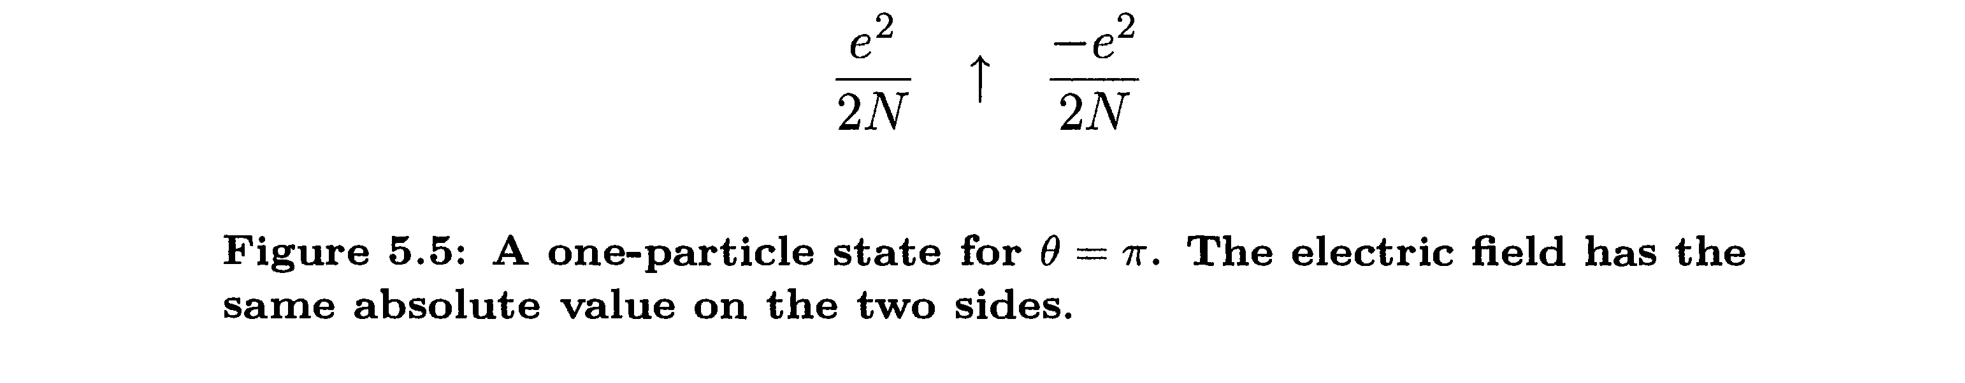
\includegraphics[width=0.76\textwidth]{figs/fig_p076_1.png}
  \caption{$\theta=\pi$ 时的一个单粒子态。电场在两侧的绝对值相同。（原文 Figure 5.5，p.76）}
  \label{fig:p076-1}
\end{figure}

请注意，在三维空间中相距 $r$ 的两个点电荷之间的 Coulomb 势正比于 $1/r$，而在一维空间中 Coulomb 势正比于 $r$。这意味着当电荷分开时势能增长，这是理解禁闭的另一种方式。

\subsection{带物质的量子理论}
% 原文 §5.7：Quantum theory with matter

现在我们要证明：只要 $\theta\neq\pi$，Lagrange 量（5.20）的量子理论中就有禁闭。这一断言就是：量子理论中每个有限能量的位形总电荷为零。

作为预备，先考虑只有物质（没有规范场）的理论。在最简单的情形 $k=N=1$，只有一个质量为 $M$ 的自由复标量场 $\phi$。这个理论的 Hilbert 空间 $\mathcal{H}_\phi$ 是 $W\oplus\overline{W}$ 的完备化对称代数（symmetric algebra），其中 $W$ 是 Poincaré 群的标量表示，质量为 $M$。存在一个使 $\phi$ 旋转的整体 $U(1)$ 对称性。相应的量子算符 $Q_\phi$，即 Noether 荷，在 $W$ 上取值为 1，在 $\overline{W}$ 上取值为 $-1$，于是在 $\mathrm{Sym}^pW\otimes\mathrm{Sym}^q\overline{W}$ 上取值为 $p-q$。这个子空间中的一个态表示 $p$ 个带正电的粒子和 $q$ 个带负电的粒子。对一般的 $k,N$，我们有 $kN$ 份这样的图像。特别地，当 $k=1$ 时存在一个整体 $SU(N)$ 对称性（在上述已经讨论过的 $U(1)$ 对称性之外）。

现在加入规范场。对于 $k=N=1$，我们有一个带单个带电标量场的 $U(1)$ 规范理论。上一段中的整体 $U(1)$ 对称性现在是局域对称性。先考虑 $\theta=0$ 的情形。对小耦合 $e^2$，我们通过量子化（5.20）的经典解构成的辛流形来构造复合系统的量子 Hilbert 空间。于是取 $\Sigma$ 为柱面 $\mathbb{R}\times S^1_V$。那么经典解的空间是 $S^1_V$ 上联络空间 $\mathcal{A}$ 的余切丛 $T^*\mathcal{A}$ 上的一个向量丛；该向量丛在平凡联络 $A=0$ 处的纤维就是 $W\oplus\overline{W}$ 底下的那个实辛向量空间。

% ===== 原文 p.77 =====
（注意，我们按复极化（complex polarization）量子化，这导致上述 Hilbert 空间 $\mathcal{H}_\phi$。）为实现规范对称性，我们必须取模去规范变换群 $\mathcal{G}$ 的辛商（symplectic quotient）。在 $S^1_V$ 上固定一个基点（无穷远点）。于是 $\mathcal{G}$ 中在基点处等于恒等的子群 $\mathcal{G}_0$ 自由地作用在 $\mathcal{A}$ 上，而商通过和乐被等同于 $U(1)$。在纯规范理论中，$T^*\mathcal{A}$ 模 $\mathcal{G}_0$ 的辛商微分同胚于 $T^*U(1)$；它的量子化 $L^2(U(1))$ 前面已经讨论过。当长度 $V\to\infty$ 时，回想唯一保持有限能量的态是真空态。经典地，真空对应于零截面，即 $T^*U(1)$ 的一个 Lagrange 子流形。常数规范变换构成的子群 $U(1)\subset\mathcal{G}$ 平凡地作用在 $\mathcal{A}$ 上——从而平凡地作用在 $T^*\mathcal{A}$ 上——因此不进入纯规范理论。在带物质的理论中，模 $\mathcal{G}_0$ 的辛商是 $T^*U(1)$ 上的一个向量丛，在恒等元处的纤维为 $W\oplus\overline{W}$。现在常数规范变换通过标量乘法非平凡地作用在纤维上。为实现这个对称性，我们有两种选择：我们可以量子化辛商，也可以考虑 Hilbert 空间中相应量子算符 $N_e$ 所湮灭的子空间。先采用后一种做法，我们看到，在无穷体积极限下，实现 $U(1)$ 之前的量子 Hilbert 空间就是 $\mathcal{H}_\phi$，因为规范场只贡献真空态。算符 $N_e$ 就等于 $Q_\phi$。因此理论的 Hilbert 空间是总电荷 $Q_\phi=0$ 的态构成的子空间。于是，正如在经典理论中一样，我们有禁闭。存在质量间隙（mass gap），最小质量为 $2M$。在小耦合理论中，定性的图像相同。

如果改为取 $W\oplus\overline{W}$ 模 $U(1)$ 的辛商，我们会被引到一个奇异空间。动量映射（moment map）是 $\mu(w,\overline{w}')=|w|^2-|\overline{w}'|^2$，而 $\mu^{-1}(0)$ 在 $(0,0)$ 处奇异。在量子化中，这个奇异点对应于真空，并且不难启发式地看出，我们会被引到与前面相同的描述。

% [Tutor Note: 这里的动量映射写作 $\mu(w,\overline{w}')=|w|^2-|\overline{w}'|^2$，第二个变量上多了一撇，疑为排印笔误：$U(1)$ 以权 $+1,-1$ 分别作用在 $W$ 与 $\overline{W}$ 上，其动量映射应写成同一个复坐标 $w$ 的 $\mu(w,\overline w)=|w|^2-|\overline w|^2$（这与正文「在 $(0,0)$ 处奇异」相容——零点集是锥面 $|w|=|\bar w|$，其顶点奇异）。若真按字面把 $w$ 与 $\bar w'$ 当作两个独立变量，$\mu^{-1}(0)$ 就是光滑流形而非奇异空间，后面的论证便不成立。另注意这里没有写出 $U(1)$ 生成元的归一化因子，它不影响零点集。]

现在允许 $\theta\neq0$。用几何量子化的语言来说，$T^*U(1)$ 上的预量子线丛（prequantum line bundle）现在被 $L_\theta\to U(1)$ 的拉回所扭化。量子态对应于给定极化的「Bohr–Sommerfeld」叶（leaves），它们是柱面 $T^*U(1)$ 中等间距的平行圆。更确切地说，若 $p$ 是余切空间中的（动量）坐标，则这些圆出现在 $p=n-\theta/2\pi$ 处，$n$ 取整数值。相应量子态的能量（在纯规范理论中）由（5.26）给出；而当 $V\to\infty$ 时我们只保留最靠近 $p=0$ 的那个（些）圆，它对应于真空态。若 $\theta\neq\pi$，这样的圆是唯一的，我们得到与上面相同的禁闭图像。对于 $\theta=\pi$，这样的圆有两个，对应于两个真空态。因此，在带物质的理论中，在模去常数规范变换之前，我们必须量子化两份不相交的 $W\oplus\overline{W}$，以得到 $\mathcal{H}_\phi\oplus\mathcal{H}_\phi$。如果像以前一样给每个真空态指定零电荷，那么对应于 $U(1)$ 对称性的算符 $N_e$ 就是 $Q_\phi\oplus Q_\phi$。被 $Q_\phi\oplus Q_\phi$ 湮灭的 $\mathcal{H}_\phi\oplus\mathcal{H}_\phi$ 的子空间，恰好是前面所见的系统的两份拷贝，每份带一个真空。这是量子理论的两个「实现」（realization），每个都有一个大小接近 $2M$ 的质量间隙。我们也可以构造包含单个电荷、能量约为 $M$ 的态，其中当 $x\to-\infty$ 时看到理论的一个实现或真空，而当 $x\to+\infty$ 时看到另一个。这些态就是在两个真空之间插值的「孤子」（soliton）；我们将在第 9 讲讨论这类态（主要是在可以用另一种拓扑论证看到它们的场合）。

% ===== 原文 p.78 =====
为论证这些启发式的图像，我们来做计算。由（5.20）可见 Hamilton 量为
\begin{equation}
  \tag{5.30}
  \label{eq:5-30}
  H=\int_{-\infty}^{\infty}dx\left(\frac{1}{2}|\pi_\phi|^2+|d_A\phi|^2+M^2|\phi|^2+\frac{N}{2e^2}|f_A|^2\right),
\end{equation}
其中 $\phi$ 是 $\mathbb{R}$ 上的场。这里 $\pi_\phi$ 是 $\phi$ 的共轭动量，$f=f_A$ 同前是曲率的 Hodge 星。我们把 $A$ 的运动方程代入，从而导出 $\phi$ 的有效 Hamilton 量。后者由（5.20）的 Lagrange 量对 $A$ 变分得到：
\begin{equation}
  \tag{5.31}
  \label{eq:5-31}
  \frac{N}{e^2}\frac{df}{dx}=j,
\end{equation}
其中流为
\[
  j=\phi\pi_\phi-\overline{\phi\pi_\phi}.
\]
我们积分（5.31）得到
\begin{equation}
  \tag{5.32}
  \label{eq:5-32}
  f(x)=\frac{e^2}{N}\left\{\int_{-\infty}^{\infty}dy\,G(x-y)j(y)+c\right\}
\end{equation}
其中 $c$ 为某个常数，而
\[
  G(x-y)=\begin{cases}1,&x\ge y;\\ 0,&x<y.\end{cases}
\]
请注意
\begin{equation}
  \tag{5.33}
  \label{eq:5-33}
  \lim_{x\to-\infty}f(x)=\frac{e^2c}{N}.
\end{equation}
代入（5.30）我们看到
\[
  H=H_0+\Delta H,
\]
其中 $H_0$ 是自由标量粒子的 Hamilton 量（若在 $A=0$ 处计算），而
\[
  \Delta H=\frac{e^2}{2N}\int_{-\infty}^{\infty}dx\left\{\int_{-\infty}^{\infty}dy\,G(x-y)j(y)+c\right\}^2.
\]
微扰项 $\Delta H$ 是非局域的，并且是奇异的。

% [Tutor Note: 由 (5.31) 到 (5.32) 用的是 $dG(x-y)/dx=\delta(x-y)$，而 $G$ 取成阶跃函数这一步同时选定了常数 $c$ 的含义：把 (5.32) 取 $x\to-\infty$ 即得 $f(-\infty)=e^2c/N$，也就是 (5.33)。注意 $G(x-y)=1$（$x\ge y$）意味着 $f(x)$ 只累积 $x$ 左侧的电荷，若把阶跃函数取成反向（$x\le y$ 时为 1），则 $c$ 会变成 $f(+\infty)N/e^2$，$c\to-c$，而 (5.34) 中 $Q_\phi+2c$ 的符号随之翻转，禁闭的判据看上去就反了。另外 $j=\phi\pi_\phi-\overline{\phi\pi_\phi}$ 与通常的 $U(1)$ 流 $i(\overline\phi\partial_t\phi-\phi\partial_t\overline\phi)$ 相差一个因子 $i$（此处 $j$ 是反厄米的）；由于 $\Delta H$ 只含 $j^2$，这个 $i$ 在能量中不起作用，但在把 (5.34) 与 $Q_\phi$ 的本征值（整数）比较时必须留意。]

现在我们必须确定使 $\Delta H$ 有限的那些态 $\Psi$ 构成的子空间。先考虑 $c=0$。这时 $\langle\Psi|\Delta H|\Psi\rangle$ 有限当且仅当
\[
  \lim_{x\to\infty}\langle\Psi|f(x)|\Psi\rangle=0,
\]
其中 $f(x)$ 由（5.32）定义。现在
\[
  \lim_{x\to\infty}\int_{-\infty}^{\infty}dy\,G(x-y)j(y)=\int_{-\infty}^{\infty}dy\,j(y)=Q_\phi
\]
是 Hilbert 空间 $\mathcal{H}_\phi$ 中的电荷算符。因此，若 $c=0$，我们就得到禁闭：
\[
  \langle\Psi|Q_\phi|\Psi\rangle=0.
\]

% ===== 原文 p.79 =====
一般地，$c$ 通过（5.33）与（5.29）同 $\theta$ 相联系：
\[
  |c|=\min_n\left(\frac{\theta}{2\pi}+n\right).
\]
这就是 $-\infty$ 处电场之值。此外，我们从 $\Delta H$ 中减去一个（无穷大的）常数，以计入无穷远处的非零能量：
\[
  (\Delta H)_{\mathrm{normalized}}=\frac{e^2}{2N}\int_{-\infty}^{\infty}dx\left[\left\{\int_{-\infty}^{\infty}dy\,G(x-y)j(y)+c\right\}^2-c^2\right].
\]
它在满足
\begin{equation}
  \tag{5.34}
  \label{eq:5-34}
  Q_\phi(Q_\phi+2c)|\Psi\rangle=0
\end{equation}
的态 $\Psi$ 上有限，即 $Q_\phi|\Psi\rangle=0$ 或 $Q_\phi|\Psi\rangle=-2c$。对于 $\theta\neq\pi$，唯一的可能是 $Q_\phi|\Psi\rangle=0$，于是我们得到禁闭。

% [Tutor Note: 上式（即 $|c|$ 的表达式）按原文图像逐字转写为 $\min_n\left(\frac{\theta}{2\pi}+n\right)$，但括号内显然漏了绝对值：$n$ 取遍全体整数时 $\frac{\theta}{2\pi}+n$ 无下界（$\to-\infty$），该 $\min$ 根本不存在。正确写法应为 $|c|=\min_{n}\left|\frac{\theta}{2\pi}+n\right|$，即取 $\frac{\theta}{2\pi}$ 到最近整数的距离；这与 (5.26) 中 $E_{\rm vac}\propto\min_n\left(n-\frac{\theta}{2\pi}\right)^2$ 的极小者一致，也才能给出后文 $c=\pm1/2$（$\theta=\pi$）与 $c=0$（$\theta=0$）的结论。此处应判为原文（或排版）笔误。]

对于 $\theta=\pi$，我们有 $c=\pm1/2$，而（5.34）对满足 $Q_\phi|\Psi\rangle=0$ 或 $Q_\phi|\Psi\rangle=\mp1$ 的态成立。正如在经典理论中一样，这给出四个扇区。我们按照电场在 $-\infty$ 与 $+\infty$ 处的值，把它们记为 $\mathcal{H}_{++},\mathcal{H}_{+-},\mathcal{H}_{-+},\mathcal{H}_{--}$。注意 $\mathcal{H}_{++}$ 中一个态的例子是相距很远的一对电荷–反电荷，各自的质量近似为 $M$。在电荷彼此分开的极限下，能量并不增加，所以人们当然愿意说这个理论不是禁闭的。如果我们取一个极限，让两个电荷中的一个位于固定位置而另一个趋于无穷远，那么在与第一个电荷距离固定处所作的一切局域测量都收敛到 Hilbert 空间 $\mathcal{H}_{+-}$（或 $\mathcal{H}_{-+}$，取决于被移到无穷远的那个电荷的符号以及它所取的方向）中的测量。类似地，把两个电荷都移到无穷远，人们可以在 $\mathcal{H}_{++}$ 中描述一列测量，它们收敛到 $\mathcal{H}_{--}$ 中的一个测量。在这个意义上，四个 Hilbert 空间都应看作是同一个故事的一部分。这是带多个真空的二维理论的一个普遍特征；它在二维以上没有类似物。

在禁闭的情形，对称群 $PSU(N)$ 起作用。在 $\theta=\pi$ 理论的扇区 $\mathcal{H}_{\pm\mp}$ 中，覆盖群 $SU(N)$ 起作用，因为单粒子态按 $SU(N)$ 的基本表示（fundamental representation）及其对偶表示变换。所以对称群是 $PSU(N)$，但 $\theta=\pi$ 时是 $SU(N)$。

$k>1$ 的故事是类似的。

\subsection{参考文献与交叉引用}

大型 $N$ 极限的讨论见 [I-Renorm Groups] 的第 4 讲、本系列的第 4 讲，以及 [I-Homework] 的习题 FE4。对称性破缺的讨论见本系列第 1 讲。

靶空间为复射影空间的 $\sigma$ 模型的大 $N$ 极限，在下列文献中被分析：

\begin{itemize}
\item A. D'Adda, M. Luscher, P. Di Vecchia, \emph{A $1/N$ expandable series of nonlinear sigma models with instantons}, Nucl. Phys. \textbf{B146} (1978), 63--76.
\item E. Witten, \emph{Instantons, the quark model, and the $1/N$ expansion}, Nucl. Phys. \textbf{B149} (1979), 285--320.
\end{itemize}

关于带质量电荷的弱耦合二维规范理论的讨论，见

\begin{itemize}
\item S. Coleman, \emph{More about the massive Schwinger model}, Annals of Physics \textbf{101} (1976), 239--267.
\end{itemize}

% [Tutor Note: 原文文献条目 "Nucl. Phys. B146 (1978), 63--76.." 末尾有两个句点，是排印重复（本文件已按惯例只保留一个）；同一条中作者名印作 "M. Luscher" 而未加变音符号，通行拼写为 Lüscher。这两处均不影响文献识别。]
